\documentclass[final]{beamer}
\usetheme{RJH}
\usepackage{color}
\usepackage{algorithm}
\usepackage{algorithmic}
\usepackage{graphicx}
\usepackage{caption}
\usepackage{subcaption}
\usepackage[orientation=landscape,size=a0,scale=1.4,debug]{beamerposter}
\usepackage[absolute,overlay]{textpos}
\setlength{\TPHorizModule}{1cm}
\setlength{\TPVertModule}{1cm}
\definecolor{likePurple}{RGB}{74,24,137}
\graphicspath{{./figures/}}
\title{Sparsity \& Surveillance}
\author{Rhian Davies (2$^{nd}$ year PhD student) supervised by: Idris Eckley \ \ \ \  Lyudmila Mihaylova  \ \ \ \ Nicos Pavlidis}
\institute{STOR-i CDT  \ \ \ \ Lancaster University}
\footer{www.lancs.ac.uk/$\sim$daviesr3}
\date{}

\begin{document}
\begin{frame}{} 

\begin{textblock}{20}(2.,0.7)

\includegraphics[width=15cm]{logoleft.png}
\end{textblock}

\begin{textblock}{20}(102.5,0.7)

\includegraphics[width=15cm]{logoright.png}
\end{textblock}

%%%%%%%%%%%%%%%%%%%%%%%%%%%%%%%%%%%%%%%%%%%%%%%%%%%%%%%%%%%%%%%%%%%%%%%%%%%%%%%%%%%%%%%%
%%%%%%%%%%%%%%% COLUMN 1 %%%%%%%%%%%%%%%%%%%%%%%%%%%%%%%%%%%%%%%%%%%%%%%%%%%%%%%%%%%%%%%%%
%%%%%%%%%%%%%%%%%%%%%%%%%%%%%%%%%%%%%%%%%%%%%%%%%%%%%%%%%%%%%%%%%%%%%%%%%%%%%%%%%%%%%%%

\begin{textblock}{36}(3,12)
\begin{block}{Motivation}

Surveillance cameras are ubiquitous in many countries, constantly collecting and storing a  \textcolor{likePurple}{\textbf{huge stream of data}}. A typical video camera will need to store \textcolor{likePurple}{\textbf{$10,368,000$ pixels every second}}. This large data mass leads to the need for  \textcolor{likePurple}{\textbf{accurate, fast and automated systems}} to convert raw video into information.

\vspace{0.5cm}

%\begin{quote}
%``Big Brother is Watching You.'' 
% \newline -  George Orwell, 1984  
%\end{quote}

\begin{figure}
        \centering
        \begin{subfigure}[b]{0.4\textwidth}
                \centering
                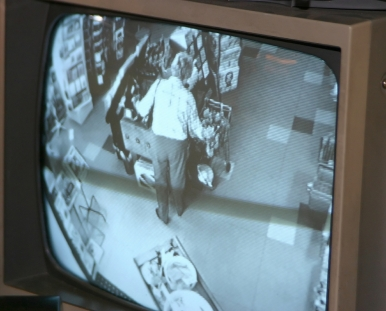
\includegraphics[height=7cm]{cctv.jpg}
                \end{subfigure}%%
        \begin{subfigure}[b]{0.4\textwidth}
                \centering
                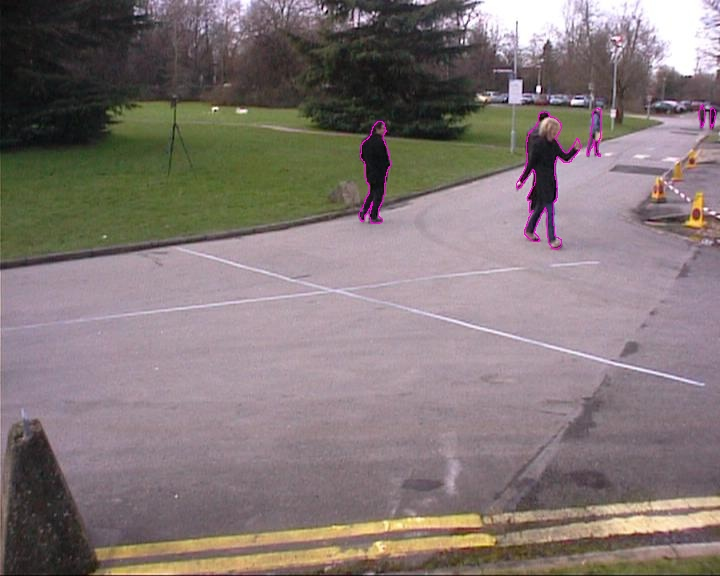
\includegraphics[height=7cm]{fgSparse}
                \end{subfigure}
\end{figure}
\vspace{0.5cm}

\textcolor{likePurple}{\textbf{The Problem: Classifying video as foreground \& background.}}
\vspace{0.5cm}

\begin{itemize}

\item Traditionally background subtraction is used, modelling the background of video and then subtracting this from the current frame. 
\item Standard background subtraction requires knowledge of every pixel. 
\item However \textcolor{likePurple}{\textbf{foreground is sparse}} both spatially and temporally. 
\item It is wasteful of resources to store and process every pixel, when we only want to learn about the sparse foreground.
\item Compressive sensing can help.
\end{itemize}
\end{block}
\end{textblock}


\begin{textblock}{36}(3,45)
\begin{block}{What is Compressive Sensing?}

\begin{columns}
\begin{column}{22cm}

Compressive sensing is a method that \textcolor{likePurple}{\textbf{reduces the amount of data collected}} from a signal without compromising the ability to later \textcolor{likePurple}{\textbf{reconstruct the signal accurately.}} This will only work if the signal is  \textcolor{likePurple}{\textbf{sparse}}. The size of the data collected is reduced from $N$ (all the pixels) to $M$.

\begin{itemize}
\item Select $M \ll N$.
\item Encode the signal $\boldsymbol{x}$ using matrix $\boldsymbol{\Phi}$. 
\item Decode the encoded signal $\boldsymbol{y}$ using recovery algorithm $\Delta$. 
\end{itemize}
\end{column}


\begin{column}{13cm}

 \begin{figure}[h]
        \centering
        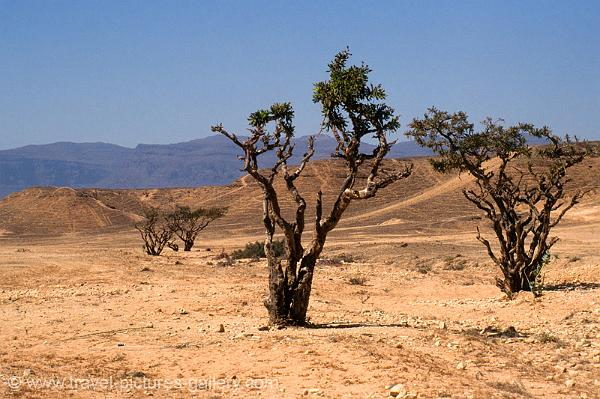
\includegraphics[width = 12cm]{sparseD.jpg}
       \end{figure}

 \begin{figure}[h]
        \centering
        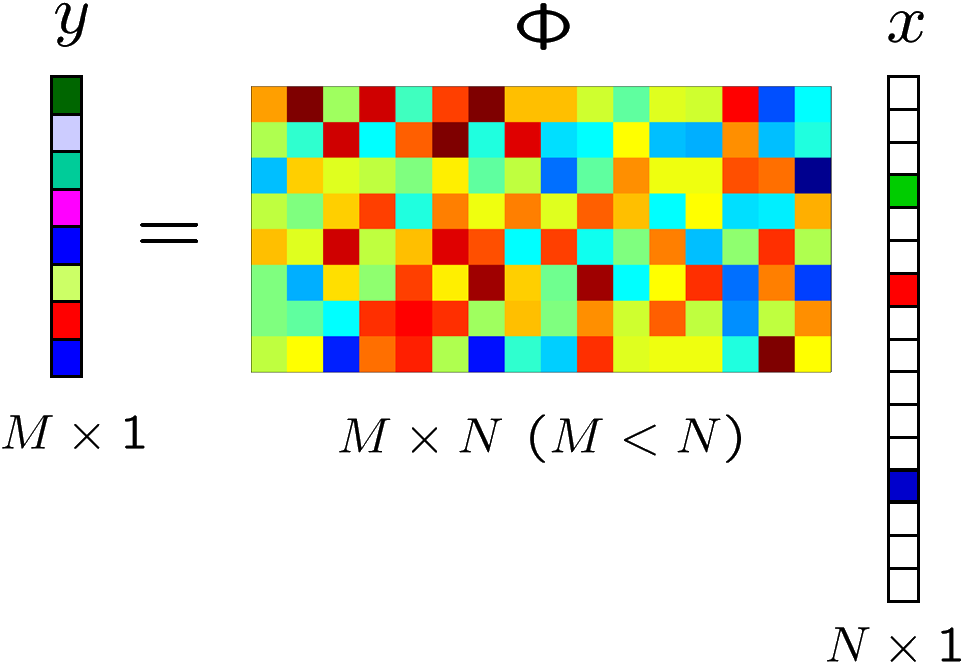
\includegraphics[width = 12cm]{csss}
       \end{figure}
\end{column}%
\end{columns}
  
\end{block}
\end{textblock}


\begin{textblock}{36}(3,66)
  \begin{block}{Compressive Sensing Background Subtraction}

    \begin{itemize}
    \item Compressively sense each frame at time $t$ \hspace{9cm} \textcolor{likePurple}{$\boldsymbol{y_t} = \boldsymbol{\Phi x_t}$.}
\item Reconstruct the foreground mask directly  \hspace{5cm} \textcolor{likePurple}{${\boldsymbol{fg_t}} = \Delta (\boldsymbol{y_t} - \boldsymbol{y^b_t})$.}
\item Update the compressed background  \hspace{3cm}  \textcolor{likePurple}{$\boldsymbol{y^b_{t+1}} = \alpha \boldsymbol{y_{t+1}} + (1 - \alpha)\boldsymbol{y^b_t}$.}
    \end{itemize}


It is possible estimate the location and shape of foreground activity based \textcolor{likePurple}{\textbf{only on the compressed background model and frame}} allowing a reduction in storage and computation at the sensor.
\vspace{0.16cm}
  \end{block}
\end{textblock}




%%%%%%%%%%%%%%%%%%%%%%%%%%%%%%%%%%%%%%%%%%%%%%%%%%%%%%%%%%%%%%%%%%%%%%%%%%%%%%%%%%%%%%%%%%
%%%%%%%%%%%%%%% COLUMN 2 %%%%%%%%%%%%%%%%%%%%%%%%%%%%%%%%%%%%%%%%%%%%%%%%%%%%%%%%%%%%%%%%%
%%%%%%%%%%%%%%%%%%%%%%%%%%%%%%%%%%%%%%%%%%%%%%%%%%%%%%%%%%%%%%%%%%%%%%%%%%%%%%%%%%%%%%%

\begin{textblock}{36}(42,12)
   \begin{table}[ht!]
\centering
%\caption{CS$_{\ell_1}$ and CS$_{\text{OMP}}$ segmentation for 3 test scenes ($N = 4096, M = 2048, \alpha = 0.05$). }

\begin{tabular}{cccc}
\parbox[top]{88mm}{Original Frame} &  \parbox[top]{88mm}{Ground Truth} & \parbox[top]{88mm}{Convex Relaxation} & \parbox[top]{88mm}{Greedy Pursuit} \\
 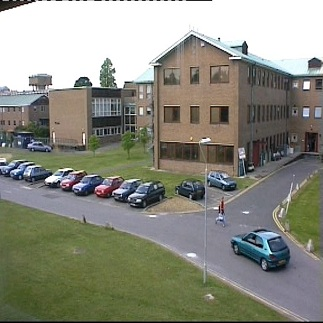
\includegraphics[width=88mm]{1}& 
\includegraphics[width=88mm]{GTB} & 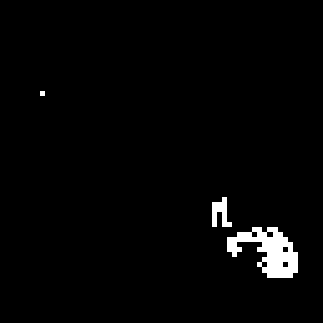
\includegraphics[width=88mm]{1l} & 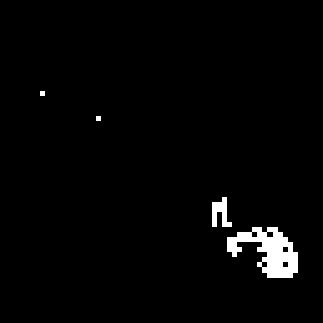
\includegraphics[width=88mm]{1o} \\
 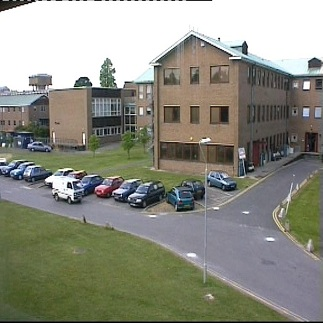
\includegraphics[width=88mm]{2}& 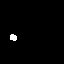
\includegraphics[width=88mm]{GTD} & 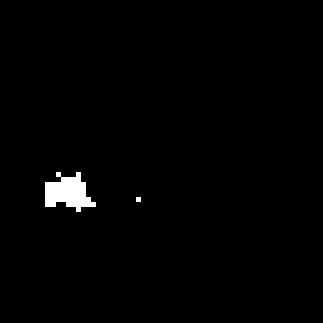
\includegraphics[width=88mm]{2l} & 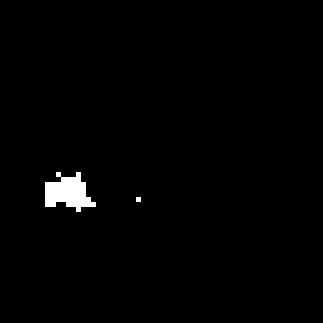
\includegraphics[width=88mm]{2o} \\
 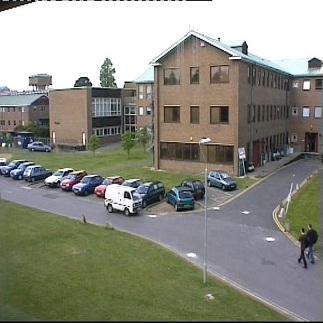
\includegraphics[width=88mm]{3}& 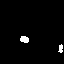
\includegraphics[width=88mm]{GTE} & 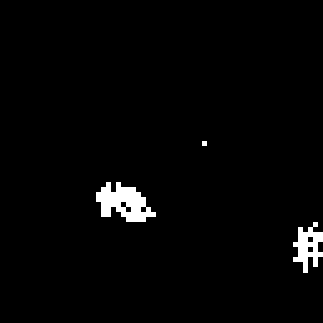
\includegraphics[width=88mm]{3l} & 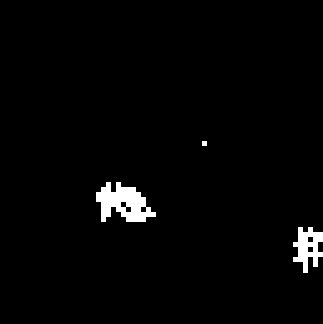
\includegraphics[width=88mm]{3o} \\
 \end{tabular}
\label{tab:gt}
\end{table}
%\end{block}
\end{textblock}

\begin{textblock}{36}(42,141)
\begin{block}{Encoding Images in a Compressed Form}
   \begin{figure}[h]
     \centering
     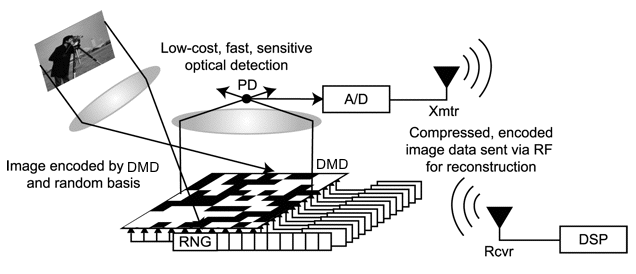
\includegraphics[width = 30cm]{spc}
     \caption{The single pixel camera}
   \end{figure}
\end{block}
\end{textblock}

\begin{textblock}{36}(42,43)
  \begin{block}{Algorithmic Approaches}
Reconstruction algorithms $\Delta$ must take the $M$ measurements in the vector $\boldsymbol{y}$, the random measurement matrix $\boldsymbol{\Phi}$ and reconstruct the size-$N$ signal $\boldsymbol{x}$. 

\begin{itemize}
\item Since $M \ll N$ there are \textcolor{likePurple}{\textbf{infinitely many solutions}} $\hat{x}$ that satisfy $\boldsymbol{y} = \boldsymbol{\Phi x} $.
\item  But we know \textcolor{likePurple}{\textbf{$\boldsymbol{x}$ is sparse}} and can use this key fact to select a solution.
\item  The \textcolor{likePurple}{$\boldsymbol{\ell_0}$\textbf{ norm}} counts the number of non-zero entries in $\boldsymbol{\hat{x}}$.
\item  We could minimize this to find a suitable solution;  
\begin{equation*}
  \label{eq:4}
 \min_{\boldsymbol{x}} ||\boldsymbol{x}||_0 \text{ subject to } \boldsymbol{y} = \boldsymbol{\Phi} \boldsymbol{x}.
\end{equation*}


\item Unfortunately solving this is \textcolor{likePurple}{\textbf{NP-complete}}.
\end{itemize}

\vspace{1cm}

There are two main alternative approaches to solving this problem. 
\begin{itemize}
\item \textcolor{likePurple}{\textbf{Convex Relaxation. }}
\newline Replaces the combinatorial problem ($\ell_0$ norm) with a convex optimization problem  ($\ell_1$ norm).  

\item \textcolor{likePurple}{\textbf{Greedy Pursuit.}}
\newline Iteratively refines a sparse solution by successively identifying one or more components that yield the greatest improvement in signal quality.
\end{itemize}
%Convex Relaxation. 
%Greedy Pursuit.

\vspace{1.5cm}
Our current work investigates the performance of these two methods in the foreground detection application. 
  \end{block}
\end{textblock}

\begin{textblock}{36}(42,141)
  \begin{block}{Restricted Isometry Property (RIP)}
     
 A matrix $\boldsymbol{\Phi}$ satisfies the (RIP) of order $K$ if there exists a $\delta_K  \in (0,1)$ such that 
\begin{equation*}
  \label{eq:40}
  (1 - \delta_k)\|\boldsymbol{x}\|^2_2 \leq\|\boldsymbol{\Phi} \boldsymbol{x}\|^2_2 \leq (1 + \delta_k)\|\boldsymbol{x}\|^2_2,
\end{equation*}

for all $\boldsymbol{x} \in \sum_K = \{\boldsymbol{x}:\|\boldsymbol{x}\|_0 \leq K\} $, \newline

where $\|\boldsymbol{x}\|_0$ is the zero pseudo-norm defined as

\begin{equation*}
\|\boldsymbol{x}\|_0 = \#(i|x_i \neq 0). 
\end{equation*}
 
If $\boldsymbol{\Phi}$ satisfies the RIP with order $2K$, then $\boldsymbol{\Phi}$ approximately preserves the distance between any pair of $K$-sparse vectors. Unfortunately the task of checking that a matrix satisfies the RIP is a NP-hard problem, but fortunately the RIP will hold true with high probability if $\boldsymbol{\Phi}$ is selected as a random matrix and $M \geq cK\log \frac{N}{K}$, where $c$ is a small constant. 

\end{block}
\end{textblock}






%%%%%%%%%%%%%%%%%%%%%%%%%%%%%%%%%%%%%%%%%%%%%%%%%%%%%%%%%%%%%%%%%%%%%%%%%%%%%%%%%%%%%%%%%%
%%%%%%%%%%%%%%% COLUMN 3 %%%%%%%%%%%%%%%%%%%%%%%%%%%%%%%%%%%%%%%%%%%%%%%%%%%%%%%%%%%%%%%%%
%%%%%%%%%%%%%%%%%%%%%%%%%%%%%%%%%%%%%%%%%%%%%%%%%%%%%%%%%%%%%%%%%%%%%%%%%%%%%%%%%%%%%%%%%%



\begin{textblock}{36}(81,12)
  \begin{block}{Convex Relaxation: $\ell_1$ minimization}
 Originally used in geophysics to aid detection of sparse spike trends in earthquake data, optimisation based on the $\ell_1$ norm can approximate sparse signals with high probability.   The $\ell_1$ norm is defined as,  
\begin{equation*}
  \|\boldsymbol{x}\|_1 = \sum_{i=1}^{N}|x_i|.
\end{equation*}
Minimising the $\ell_1$ norm \textbf{\textcolor{likePurple}{determines the simplest solution}} $x$ in terms of the $\ell_1$ norm which explains the observations. 

\begin{equation*}
 \label{eq:4}
 \min_{\boldsymbol{x}} ||\boldsymbol{x}||_1 \text{ subject to } \boldsymbol{y} = \boldsymbol{\Phi} \boldsymbol{x}.
\end{equation*}
  \end{block}
  
\end{textblock}

\begin{textblock}{36}(81,32)
  \begin{block}{Greedy Pursuit: Orthogonal Matching Pursuit (OMP)}



\begin{itemize}
\item OMP iteratively computes local optimum solutions in the hope that these will lead to the global optimum solution. 
\item Each iteration it determines the column of $\boldsymbol{\Phi}$ which is most correlated with $\boldsymbol{y}$.
\item It uses this column to estimate one component of the solution $\boldsymbol{x}$.
\item This is repeated until it reaches some user-defined stopping criterion. 
\item The \textbf{\textcolor{likePurple}{number of iterations is key}} to the performance of the algorithm, both in terms of signal quality and computational time.
\end{itemize}

\end{block}
\end{textblock}

\begin{textblock}{36}(81,49)
  \begin{block}{Results}
    \begin{figure}
        \centering
        \begin{subfigure}[b]{0.4\textwidth}
                \centering
                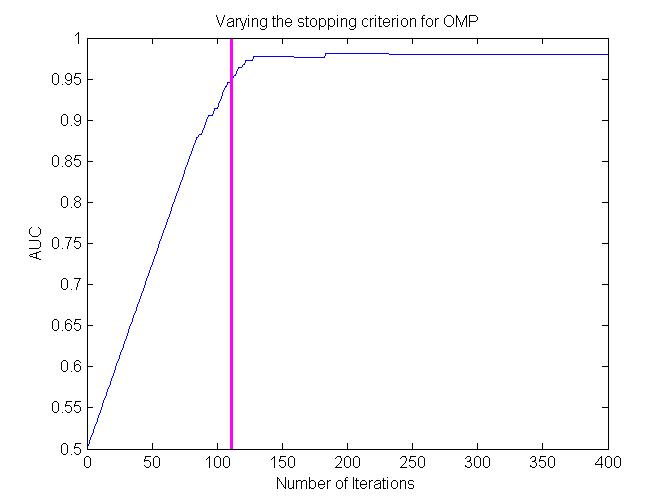
\includegraphics[height=14cm]{varyingSComp}
                \caption{Stopping criterion for OMP}
               % \label{fig:gull}
        \end{subfigure}%%
        \begin{subfigure}[b]{0.4\textwidth}
                \centering
                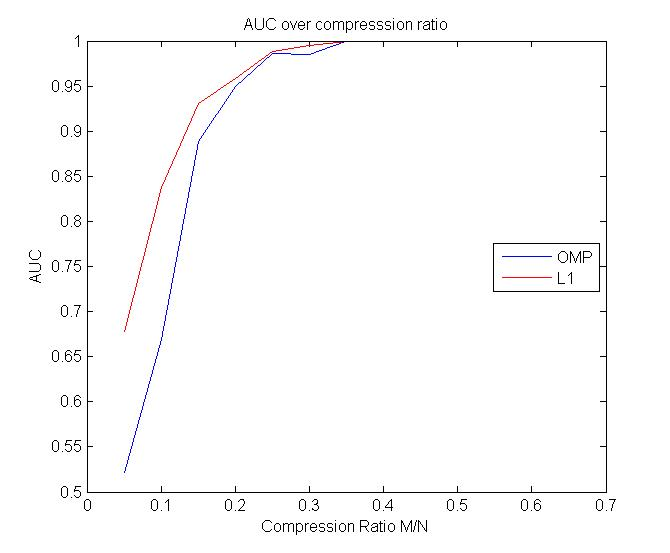
\includegraphics[height=14cm]{AUCcompressionRatio}
                \caption{AUC for  Sparsity Ratios}
              %  \label{fig:tiger}
        \end{subfigure}
\end{figure}
  \end{block}
\end{textblock}




\begin{textblock}{36}(81,69)
  \begin{block}{Conclusion and Future Plans}
   \begin{itemize}
  \item $\ell_1$ minimisation outperforms OMP, but it's close!
\item The stopping criterion is vital for OMP - adaptive methods needed?
\item Ideal boundaries for compression ratio of $\frac{M}{N}$ around $25 \% - 35 \%$ 
\item Can we incorporate spatial information to aid the recovery process?
  \end{itemize}
 \end{block}
\end{textblock}

\end{frame}
\end{document}


%%%%%%%%%%%%%%%%%%%%%%%%%%%%%%%%%%%%%%%%%%%%%%%%%%%%%%%%%%%%%%%%%%%%%%%%%%%%%%%%%%%%%%%%%%
%%%%%%%%%%%%%%% END %%%%%%%%%%%%%%%%%%%%%%%%%%%%%%%%%%%%%%%%%%%%%%%%%%%%%%%%%%%%%%%%%
%%%%%%%%%%%%%%%%%%%%%%%%%%%%%%%%%%%%%%%%%%%%%%%%%%%%%%%%%%%%%%%%%%%%%%%%%%%%%%%%%%%%%%%%%%



 








\begin{textblock}{36}(3,42)
  \begin{block}{Sparse and Compressible Signals}
  \begin{itemize}
  \item A signal is known as being \textbf{K-sparse} if $\boldsymbol{x} \in R^N$ can be represented as a linear combination of $K$ basis vectors. 
   \item Interested in $K \ll N$.
     \item If a signal is \textbf{compressible} there exist $K$ large coefficients but the remaining $N-K$ coefficients are only required to be small and not necessarily zero. 
  \end{itemize}
 
\begin{figure}
        \centering
        \begin{subfigure}[b]{0.4\textwidth}
                \centering
                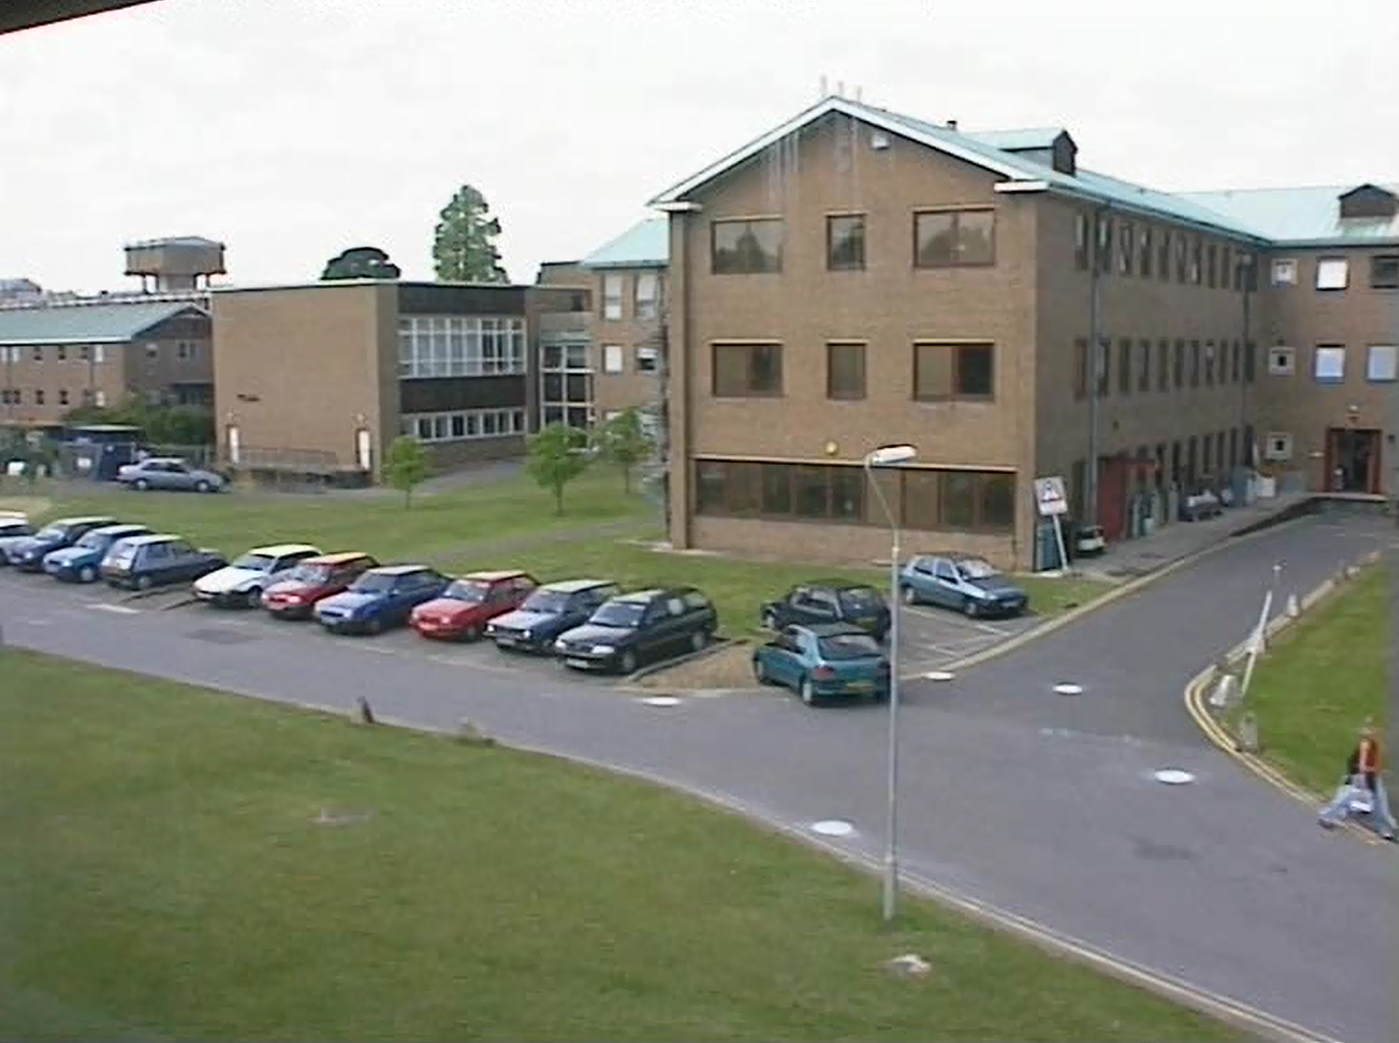
\includegraphics[width=5cm]{camReal}
                \caption{Test frame}
               % \label{fig:gull}
        \end{subfigure}%
        \begin{subfigure}[b]{0.4\textwidth}
                \centering
                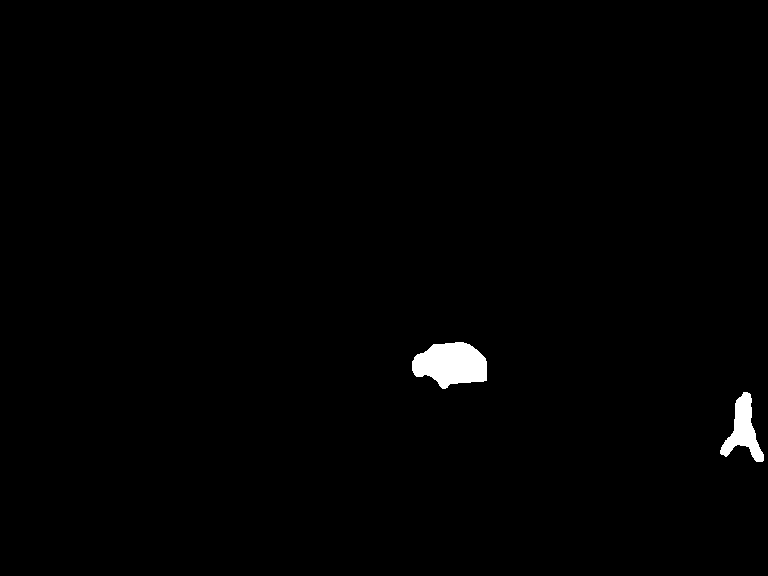
\includegraphics[width=5cm]{camGT}
                \caption{Ground truth}
              %  \label{fig:tiger}
        \end{subfigure}
\caption{The spatial sparsity of foreground. A frame from the PETS data set and the corresponding foreground in white. In this example, less than 1\% of the frame is foreground, as N=442,368 and K=3862. }\label{fig:sparse}
\end{figure}

  \end{block}
\end{textblock}


\begin{algorithm}[H]
\caption{Orthogonal Matching Pursuit}  
\begin{algorithmic}
\STATE{Define the columns of $\boldsymbol{\Phi}$ to be $\varphi_1, \varphi_2, \hdots, \varphi_N$.}% each of length $M$.}
\REQUIRE $\boldsymbol{r_0} = \boldsymbol{y}, \Lambda_0 = \emptyset$ and iteration counter $i = 1$
\FOR{$i < T$} % \COMMENT{T is the maximum iteration count.}
 \STATE  $\lambda_t = \text{argmax }_{j=1,\hdots,N}|<r_{t-1}, \varphi_j>|$ \\  \COMMENT{Find the index for the column of $\Phi$ with the greatest contribution.}
 \STATE  $\Lambda_t = \Lambda_{t-1} \cup {\lambda_t}$, $\Phi_t = [\boldsymbol{\Phi_{t-1}}, \varphi_{\lambda_t}]$ \\ \COMMENT{Keeps track of the columns used.}
\STATE   $\boldsymbol{x_t} = \text{argmin}_{\boldsymbol{x}} || \boldsymbol{y} - \boldsymbol{\Phi_t} \boldsymbol{x}||_2$  \\ \COMMENT{Updates the signal estimate.}
\STATE  $\boldsymbol{r_t} =  \boldsymbol{y} - \boldsymbol{\Phi_t} \boldsymbol{x_t}$ \\ \COMMENT {Updates the measurement residual.}
\ENDFOR
\RETURN  $\boldsymbol{\hat{x}}$
\end{algorithmic}
\end{algorithm}






